\section{Introduction}
\label{sec:introduction}

Airline disruption recovery is a continuous operational allocation problem. After disruptions occur, airline operations control centers (AOCCs) must determine which affected flight chains deserve immediate attention, which disruptions require more detailed diagnosis, and where recovery effort should ultimately be deployed under limited time, analytical capacity, and operational resources. Effective recovery support therefore requires more than identifying disruption severity: it must translate progressively available operational information into signals that are matched to the recovery decision being made.

Delay provides a natural baseline for this task. It is interpretable and continuously updated, making it well suited to rapid operational screening. In the decision-time comparisons of this study, the scalar delay priority is the expected successor take-off delay conditional on information then available, rather than the delay eventually observed after the flight is completed. Yet disruption consequences are not determined by delay magnitude alone. As aircraft-linked flight chains evolve, realized predecessor operations, turnaround conditions, and successor states progressively clarify the operating situation. Passenger, route, and downstream exposure references already available at the decision time may also distinguish the consequences of similarly delayed chains. Existing airline recovery research has documented the multidimensional nature of flight, passenger, and network consequences
\citep{bratuFlightOperationsRecovery2006,arikanIntegratedAircraftPassenger2016,clausenDisruptionManagementAirline2010,hassanAirlineDisruptionManagement2021}.
The relevant question is therefore not simply whether richer operating information describes more detail than delay, but how much incremental decision value those additional state and consequence distinctions provide.

Information value also depends on the recovery decision being supported. Stage-I screening allocates limited review attention across disrupted flight chains, whereas subsequent local recovery evaluates whether a shortlisted chain should receive additional recovery effort and which recovery target should be selected. Existing staged-recovery studies similarly distinguish prioritization, affected-flight identification, and subsequent recovery or schedule adjustment
\citep{peiDecisionSupportIrregular2021,jiFlightPrioritiesRecovery2021,zhaoTwoStageAircraftRecovery2023,zhongIntegratedRecoveryPriority2024}.
In our framework, screening is based on relative baseline consequence exposure, while local recovery weighs the remaining recoverable opportunity against the effort required to pursue it. A disruption may consequently warrant high screening priority without retaining a beneficial local-recovery opportunity, and information that leaves the shortlist unchanged may still alter the downstream recovery target. These distinct comparisons make the value of operating information specific to the decision being supported. Figure~\ref{fig:decision_context} illustrates this staged structure.

\begin{figure}[pos=t]
    \centering
    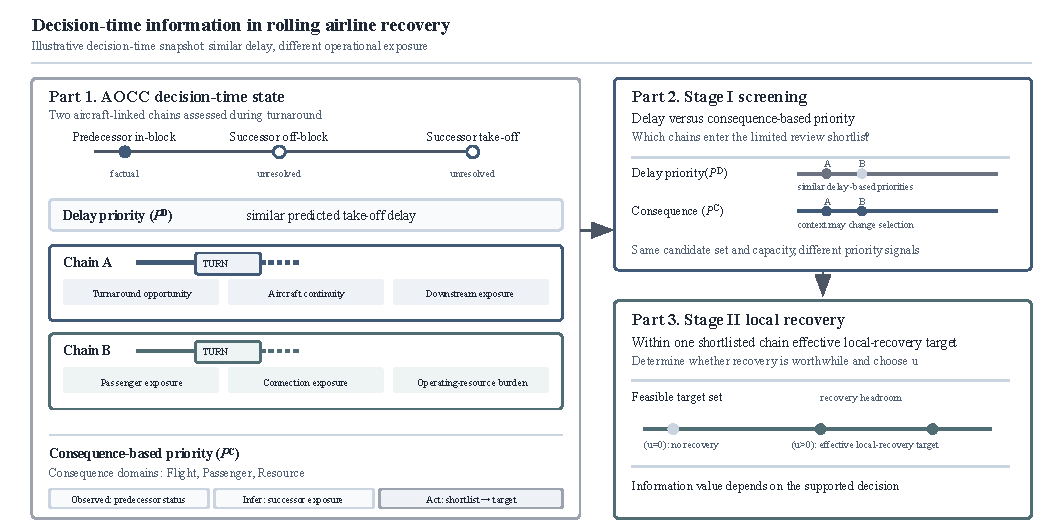
\includegraphics[width=\linewidth]{figures/figure1.pdf}
    \caption{Decision-time information and linked recovery decisions in an aircraft-linked disruption setting. Progressively revealed operating information can distinguish flight chains beyond observed delay, first affecting capacity-constrained screening across chains and subsequently informing effective local-recovery targeting within shortlisted actionable chains.}
    \label{fig:decision_context}
\end{figure}

The representation of operational information provides a second source of variation in decision value. Temporal information can retain either the current operating state alone or the trajectory through which that state was reached. Likewise, unresolved future states can be compressed into a deterministic estimate or represented in forms that preserve different aspects of uncertainty. Existing research on delay propagation and dynamic recovery has emphasized temporal evolution, aircraft rotations, and historical operating information
\citep{fleurquinSystemicDelayPropagation2013,li2021delayNetwork,erdemAirlineDelayPropagation2024},
while probabilistic approaches retain multiple possible future realizations rather than collapsing uncertainty to a single point estimate
\citep{wooScenarioBasedStochastic2021,zoutendijkProbabilisticFlightDelay2021,ogunsinaRelationalDynamicBayesian2022,dalmauProbabilisticPretacticalArrival2024}.
We examine these distinctions through Current versus History information and Point, Marginal, and Joint representations of unresolved aircraft-linked states.

Richer representation need not produce proportional decision refinement: incremental value arises when the additional distinctions retained by a representation alter the comparison relevant to the supported decision. For screening, this may involve the relative positions of flight chains near a fixed review-budget boundary. For local recovery, it may involve the consequence--effort trade-off between feasible recovery targets. Managerial objectives, nonlinear consequence thresholds, dependence among operating states, and remaining recovery headroom can affect whether a representational difference changes the preferred target. Accordingly, we evaluate not only whether information representations lead to different choices but also the model-relative loss of those choices under a common reference criterion.

Against this background, this study asks the following overarching research question:

\begin{quote}
\emph{In rolling airline recovery, how much incremental decision value does aircraft-linked operating information beyond delay provide, and how does this value vary with progressively revealed operating states, information representations, and the recovery decisions being supported?}
\end{quote}

The question has two linked dimensions. The first concerns operating information and its representation: what distinctions are added by realized milestones, historical trajectories, and alternative representations of unresolved uncertainty beyond a compact delay signal. The second concerns the supported recovery decision: whether these distinctions affect cross-chain screening, within-chain local-recovery targeting, or both. Managerial objectives, decision boundaries, and operating conditions are examined as conditions that may explain variation in incremental decision value. In this sense, decision-specific information sufficiency is an interpretation of the comparisons---whether a more compact representation preserves the distinctions needed for a particular choice---rather than a presumption that richer representations must always be preferable.

To investigate this question, we develop a unified state--consequence--decision framework with two linked recovery stages. Stage I considers fixed-budget screening, where limited review attention is allocated across disrupted aircraft-linked flight chains using expected-delay or multidimensional-consequence priorities. A delay-plus-exposure comparator helps distinguish the role of historical exposure references from that of a scalar delay signal. Stage II selects an effective local-recovery target for a chain with valid recovery support under a common multidimensional consequence--effort objective. Controlled Current--History and Point--Marginal--Joint comparisons assess how temporal information and uncertainty representation affect these decisions. Additional comparisons of managerial objectives, state-dependence mechanisms, and decision boundaries examine when the information differences become relevant to local recovery. All comparisons assess model-relative decision value under defined reference criteria, not observed causal effects of recovery actions.

The empirical design covers six independent operating years in U.S. aviation from 2017 to 2022, using consistent aircraft-linked chain definitions, recovery tasks, and within-year chronological held-out evaluation. This window includes pre-pandemic operations (2017--2019), the COVID-19 disruption period (2020), and the subsequent operational recovery period (2021--2022). The frozen 2019 evaluation remains a traceable original benchmark, while the six year-specific evaluations form the intended evidence base for the main comparisons and their variation across operating conditions.

% SIX-YEAR EMPIRICAL FINDINGS TO INSERT AFTER THE E1--E4 RUNS AND AUDIT.
% Organize in three evidence-backed parts: (i) incremental screening value of
% consequence information beyond expected delay; (ii) recoverable opportunity
% and temporal/probabilistic representation effects across the two decisions;
% (iii) roles of managerial objectives, state dependence, decision boundaries,
% and operating conditions. Report zero or mixed effects where observed.
% Do not promote the original 2019 findings to six-year conclusions.

The study makes three contributions. First, it moves the comparison of delay and multidimensional consequences beyond population-level association to operational decision substitutability. By linking screening choices to fixed review budgets, consequence coverage, and the active selection boundary, and by adding a delay-plus-exposure comparator, the analysis evaluates the incremental value of consequence distinctions for allocating limited managerial attention. Second, it distinguishes baseline consequence priority from remaining recoverable opportunity while examining the decision effects of temporal history and uncertainty representation within the same aircraft-linked operating process. The Current--History and Point--Marginal--Joint contrasts allow incremental information value to be evaluated across both screening and local-recovery tasks under common reference criteria, rather than inferred from predictive accuracy alone. Third, it relates the decision-boundary interpretation of incremental information value to managerial objectives, state-dependent recovery opportunities, and operating conditions. Through controlled objective and dependence comparisons together with year-specific evaluations, the analysis examines when simpler representations preserve the distinctions needed for recovery decisions and when additional information can change those choices.

The remainder of the paper is organized as follows. Section~\ref{sec:related_work} reviews the related literature and positions the study around operating consequences, rolling information, and decision value. Section~\ref{sec:methodology} defines the aircraft-linked operating state, multidimensional consequences, two-stage recovery decisions, and the reference criteria for incremental decision value and information sufficiency. Section~\ref{sec:implementation} presents the six-year empirical design, state reconstruction, consequence construction, decision implementation, and controlled comparisons. Section~\ref{sec:results} reports the evidence on screening, recoverable opportunity, information representations, managerial objectives, and operating-stage and regime differences. Section~\ref{sec:discussion} discusses decision-specific information value, implications for AOCC decision support, and applicability. Section~\ref{sec:conclusion} concludes.
